\documentclass[hidelinks]{article}
%
%%%%%%%%%%%%%%%%%%%%%%%%%%%%%%%%%%%%%%%%%%%%%%%%%%%%%%%%%%%%%%%
% START CUSTOM INCLUDES & DEFINITIONS
%%%%%%%%%%%%%%%%%%%%%%%%%%%%%%%%%%%%%%%%%%%%%%%%%%%%%%%%%%%%%%%
%
\usepackage{amsmath}
\usepackage{parskip} %noident everywhere
\usepackage{hyperref} % Show hyperlinks - claudio
\hypersetup{
    colorlinks = true
    linkcolor = blue
    urlcolor = red
    }
% Block diagrams
\usepackage{tikz}
\usetikzlibrary{shapes.geometric, arrows, calc}
\tikzstyle{block} = [rectangle, draw,
    text centered, rounded corners, minimum height=3em, minimum width=6em]
\tikzstyle{sum} = [draw, circle, node distance=1cm]
\tikzstyle{input} = [coordinate]
\tikzstyle{output} = [coordinate]
\tikzstyle{arrow} = [draw, -latex']
%
%%%%%%%%%%%%%%%%%%%%%%%%%%%%%%%%%%%%%%%%%%%%%%%%%%%%%%%%%%%%%%%
% END CUSTOM INCLUDES & DEFINITIONS
%%%%%%%%%%%%%%%%%%%%%%%%%%%%%%%%%%%%%%%%%%%%%%%%%%%%%%%%%%%%%%%
%
\pdfobjcompresslevel=0
%
\title{\vspace{-4cm} Submarine Mission Report}
\author{\vspace{-2cm} Claudio Vestini}
\date{}
\begin{document}
\maketitle
%
\paragraph{Motivation}
This brief report will concern the B1 submarine coding practical, where
we were tasked with designing the controller to guide a Submarine through its cave mission by tracking a given reference to avoid collisions with the cave boundaries.
Preliminary steps taken before starting development:
%
\begin{enumerate}
    \item Create and activate a virtual environment with the given requirements (numpy, matplotlib and pandas packages).
    \item Fork project repository to my GitHub account.
    \item Set up a .env file to add local packages onto Python PATH.
    \item Make sure running files do not give any errors before branching off `main'.
\end{enumerate}
%
\paragraph{Mission Data}
The first task was to obtain mission data from the given .csv file. I achieved this through the following steps:
%
\begin{enumerate}
    \setcounter{enumi}{4}
    \item Create a new branch to modify the Mission class within.
    \item Implement a new classmethod to extract each column of the mission.csv file into a separate variable, then return the data as an instance of the Mission class.
    \item Test the new functionality by using the Trajectory class's plotting methods; then merge the branch back into `main', and delete the unused branch.
\end{enumerate}
%
\paragraph{Controller}
The design of the controller necessitated a thorough understanding of the Submarine and ClosedLoop classes, both of which were to be modified.
For full analysis, check Apppendix~\ref{appendix}. I completed my implementation as follows:
%
\begin{enumerate}
    \setcounter{enumi}{7}
    \item Create a new branch to avoid pushing error prone code to `main'.
    \item Add a new method to the Submarine class to obtain the state space dynamics via matrices $A$, $B$, $C$ and $D$.
    \item Inside of a new module named control.py, create a new Controller class, initialised with the four matrices above. Create a subclass PDController, which inherits the dynamics, and possesses additional class variables $K_P$ and $K_D$. For this subclass, develop a class method to compute the next control action $u[t]$ given observation $y[t]$ and reference $r[t]$.
    \item Modify the ClosedLoop class to correctly call the controller within the simulate method.
    \item Test the controller by using the given demo.ipynb file. Merge and delete the branch.
\end{enumerate}
My decision to use a hierarchical class system proved effective as it kept the codebase modular. It also allows for future development of any other type of controller: I subsequently developed another subclass MPCController, which was better at tracking the reference but required more computational effort.
%
\newpage
\appendix
\section{System Equations} \label{appendix}
To implement the controller, I first analysed the given code to infer the system's dynamics. The submarine progresses at constant speed in the $x$ direction, so needs only be controlled in the y direction (another hint to this is that we only have one set of reference values).
\par By inspection of the transition method, given drag $D$, velocity $\frac{dy}{dt}$, actuator gain $K$, input $u(t)$ and disturbance $d(t)$, the force in the vertical direction is given by:
%
\begin{equation}
    F_y = - D \cdot \frac{dy}{dt} + K \cdot [u(t) + d(t)] \label{eq:force}
\end{equation}
%
\par Combining \eqref{eq:force} with Newton's second law we obtain acceleration:
%
\begin{equation}
    \frac{d^2y}{dt^2} = -\frac{D}{m} \cdot \frac{dy}{dt} + \frac{K}{m} \cdot [u(t) + d(t)] \label{eq:accelleration}
\end{equation}
%
\par It is then very simple to obtain all matrices for the (continuous) state space dynamics of the Plant in canonic form:
\begin{equation}
    \begin{aligned}
        \dot{x}(t) &= A x(t) + B [u(t) + d(t)] \\
        y(t) &= C x(t) + D u(t) \label{eq:plant}
    \end{aligned}
\end{equation}
%
as:
%
\begin{equation}
    \displaystyle
    A = \begin{bmatrix}
            0 & 1 \\
            0 & -\frac{D}{m}
        \end{bmatrix}; \quad
    B = \begin{bmatrix}
            0 \\
            \frac{K}{m}
        \end{bmatrix}; \quad
    C = \begin{bmatrix}
            1 \\
            0
          \end{bmatrix}; \quad
    D = \begin{bmatrix}
            0
        \end{bmatrix} \label{eq:matrices}
\end{equation}
%
\par Our system operates in discrete time, hence the PD Controller takes the standard form:
%
\begin{equation}
u[t] = K_P \cdot e[t] + K_D \cdot (e[t] - e[t-1]) \label{eq:controller}
\end{equation}
%
\par The system diagram in discrete time is then:
%
\begin{center}
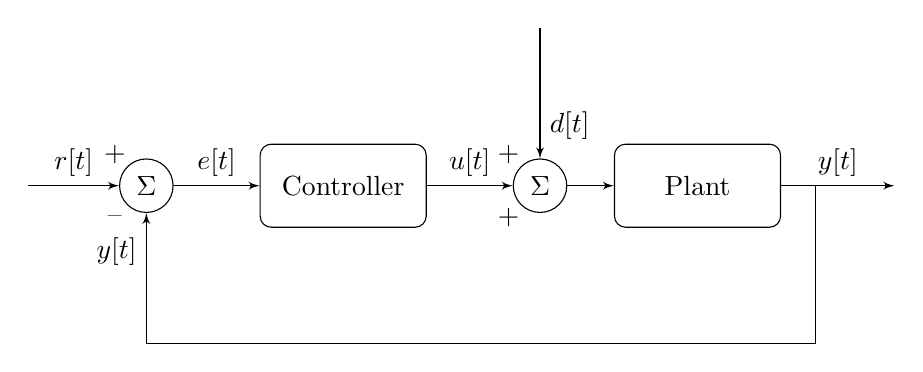
\begin{tikzpicture}[auto, node distance=2cm]
    % Nodes
    \node [input] (input) {};
    \node [sum, right of=input, node distance=1.5cm] (sum) {$\Sigma$};
    \node [block, right of=sum, node distance=2.5cm] (controller) {Controller};
    \node [sum, right of=controller, node distance=2.5cm] (sum2) {$\Sigma$};
    \node [block, right of=sum2, node distance=2cm] (plant) {Plant};
    \node [coordinate, right of=plant, node distance=1.5cm] (feedback) {};
    \node [output, right of=plant, node distance=2.5cm] (output) {};
    
    % Disturbance input node
    \node [input, above of=sum2, node distance=2cm] (disturbance) {};

    % Labels for summing junctions
    \node at ($(sum) + (-0.4,0.4)$) {+}; % Plus sign at r[t] input
    \node at ($(sum) + (-0.4,-0.4)$) {--}; % Minus sign at y[t] input
    \node at ($(sum2) + (-0.4,0.4)$) {+}; % Plus sign at d[t] input
    \node at ($(sum2) + (-0.4,-0.4)$) {+}; % Plus sign at u[t] input
    
    % Arrows
    \draw [arrow] (input) -- node {$r[t]$} (sum);
    \draw [arrow] (sum) -- node {$e[t]$} (controller);
    \draw [arrow] (controller) -- node {$u[t]$} (sum2);
    \draw [arrow] (sum2) -- node {} (plant);
    \draw [arrow] (plant) -- node {$y[t]$} (output);
    \draw [arrow] (disturbance) -- node [near end] {$d[t]$} (sum2);
    
    % Feedback
    \draw [arrow] (feedback) |- ++(0,-2) -| node[pos=0.85] {$y[t]$} (sum);
    
\end{tikzpicture}
\end{center}
\vspace{0.2cm}
where the Plant is specified in equations~\eqref{eq:plant} and~\eqref{eq:matrices} and the Controller is given by equation~\eqref{eq:controller}, with gains $K_P = 0.15$ and $K_D = 0.6$ (as per requirements).
%
\end{document}